\documentclass[11pt,a4paper]{article}
\usepackage[T1]{fontenc}
\usepackage[utf8]{inputenc}
\usepackage{lmodern}
\usepackage[margin=25mm]{geometry}
\usepackage{amsmath,amssymb,booktabs,longtable,array,graphicx}
\usepackage{xcolor,listings}
\usepackage[numbers,sort&compress]{natbib}
\usepackage[breaklinks=true,colorlinks=true,linkcolor=blue,citecolor=blue,urlcolor=blue]{hyperref}
\usepackage{url}
\usepackage{microtype}
\setlength{\emergencystretch}{2em}
\lstset{basicstyle=\ttfamily\small,columns=fullflexible,breaklines=true,frame=single,showstringspaces=false}
\newcommand{\hex}[1]{\texttt{0x#1}}
\newcommand{\code}[1]{\texttt{\detokenize{#1}}}
\newcommand{\qmax}{Q_{\mathrm{max}}}
\newcommand{\fcc}{C_{\mathrm{FCC}}}
\newcommand{\design}{C_{\mathrm{design}}}
\title{From ACPI Misreporting to an EC-Mediated Fuel-Gauge Interface:\\A Dell Venue 10 Pro 5055 Case Study}
\author{Krzysztof Jakóbczyk}
\date{31 October 2026\\\small Research preprint draft; single-device case study}
\hypersetup{pdftitle={From ACPI Misreporting to an EC-Mediated Fuel-Gauge Interface},pdfauthor={Krzysztof Jakóbczyk}}
\begin{document}
\maketitle
\begin{abstract}
Battery health reported by an operating system can conflate firmware defects, stale information, and fuel-gauge model state. We document an owner-authorized investigation of one Dell Venue 10 Pro 5055 running Linux. Starting from inconsistent ACPI telemetry, we identify an incorrect voltage source in the battery status method and validate a six-byte AML override across a reboot. Boardview analysis and unsuccessful direct gauge probes motivate investigation of the embedded controller (EC). Offline extraction of official Dell A04 and A07 update packages yields byte-identical 128-KiB EC images. CR16C analysis connects embedded battery-programming scripts to an internal transaction engine and reveals a host-accessible register interface to that engine. We validate the interface against live gauge measurements and acquire 25 checksum-verified DataFlash blocks. A separately authorized experiment changes only the active profile's stored maximum chemical-capacity parameter, from 7720 to 8794 mAh, followed by one gauge reset. Reported full-charge capacity increases from 5973 to 6827 mAh and reported state of health from 78\% to 95\%, while the cycle count remains 49 and both profile-0 resistance-table blocks remain byte-identical. These are model-reporting changes, not evidence of electrochemical capacity recovery. We release an auditable evidence structure, offline verification tools, protocol details, and the limitations of this single-subject intervention.
\end{abstract}

\section{Introduction}
Battery telemetry is a chain of interpretations. Physical cells feed a measurement and estimation circuit; platform firmware aggregates its output; ACPI describes an operating-system interface; the kernel exports quantities used by desktop applications. A plausible percentage at the end of this chain does not establish which layer produced it. Conversely, an implausible percentage is not sufficient evidence of worn cells.

This case began with inconsistent Linux battery values on an aging convertible tablet. The investigation subsequently crossed four boundaries: ACPI semantics, board-level connectivity, proprietary EC firmware, and the fuel gauge's persistent model state. The resulting access path required neither opening the tablet nor adding an external bus adapter. This is a platform-specific reverse-engineering result, not a claim that arbitrary Dell systems expose the same interface.

The work makes four bounded contributions:
\begin{enumerate}
\item A reproducible diagnosis and boot-time validation of an ACPI battery-voltage defect, separated from an unresolved information-refresh issue.
\item An evidence chain from boardview connectivity and vendor update packages to a statically reconstructed, dynamically exercised EC-mediated fuel-gauge interface.
\item A documented transport, register map, and checksum-verified acquisition of configuration and learned-state data.
\item A tightly scoped persistent-parameter intervention with full-block comparison and a transaction audit, together with an explicit account of causal and physical-capacity limitations.
\end{enumerate}

All observations concern one owner-controlled device. The paper neither reports a security-boundary bypass nor claims to have discovered a universal battery-reset mechanism. Root-level userspace access was already available. The gauge reported an unsealed access state before the persistent experiment, and no unseal keys were sent.

\section{Terminology and evidence model}
\subsection{Capacity, health, and units}
We distinguish four quantities throughout the paper. \emph{Design capacity} is a configured reference, here 8680 mAh. \emph{Qmax} is a learned or configured maximum chemical-capacity parameter. \emph{Full-charge capacity} (FCC) is the gauge's predicted deliverable charge under its load, temperature, resistance, and termination model. \emph{State of health} (SOH) is a separate gauge-reported estimate under reference conditions. The specific gauge exposes these quantities through documented interfaces~\cite{ti-trm}.

The two commonly displayed percentages are therefore not interchangeable:
\begin{equation}
 H_{\mathrm{FCC}}=100\frac{\fcc}{\design},\qquad W_{\mathrm{FCC}}=100-H_{\mathrm{FCC}}.
\end{equation}
A different shorthand, $100-\mathrm{SOH}$, uses a different model output. Neither expression measures irreversible physical deterioration independently of the gauge. Charge in mAh is also not energy in Wh: actual energy requires integration of voltage and current over time. No such independent discharge-energy experiment was performed here.

Linux power-supply properties use scaled units~\cite{linux-battery}. A returned value of \code{voltage_now=5973000} is interpreted as 5.973 V, even when its numerical origin was a 5973-mAh charge value. This distinction becomes central to the initial defect.

\subsection{Address spaces}
The paper keeps four namespaces separate: seven-bit I$^2$C addresses; eight-bit address bytes including the direction bit; logical EC registers and block commands; and file offsets in the extracted EC image. The EC's seven-bit address is \hex{10}; its write/read address bytes are \hex{20}/\hex{21}. The gauge's seven-bit address is \hex{55}; its normal write address byte is \hex{AA}. A logical EC register \hex{18} is not a gauge register \hex{18}, and firmware offset \hex{83B6} is neither kind of bus address.

SMBus word replies are decoded in transfer order as little-endian words. Multi-byte fields inside the acquired DataFlash blocks are interpreted with the field layout's big-endian storage convention. The Qmax experiment explicitly tests this distinction: the stored bytes change from \code{1e 28} to \code{22 5a}.

\subsection{Evidence hierarchy}
We distinguish \emph{observed} bus replies and file bytes, \emph{statically inferred} control flow, and \emph{unmeasured} physical behavior. A valid transport CRC verifies a received frame, not a fuel-gauge algorithm. A passing byte-comparison assertion verifies the comparison encoded by that assertion, not the correctness of every disassembly inference. An extracted vendor image matching another extracted vendor image does not establish that the running EC's entire memory is identical.

The companion repository assigns evidence identifiers to these claims. Its manifest preserves source and released-artifact SHA-256 digests, including explicit transformations for normalized local paths and removal of the sysfs serial-number field. Wire payloads and measured DataFlash blocks remain intact. Vendor firmware, boardview source files, and third-party binaries are not redistributed.

\section{Experimental platform and procedure}
\subsection{Device and authorization}
The subject was a Dell Venue 10 Pro 5055, DMI board identifier \code{084N67}, running BIOS A04. The study host reported Ubuntu 26.10 and kernel \code{7.3.0-9-generic}. The boardview identified platform 14238-1, a \code{BQ27510DRZR-G3-GP} at PU4401, and a \code{NPCE948LA0BX-GP} EC at U4101. These strings identify design components, not an independently inspected silicon marking.

The owner authorized progressively broader operations: initial readout, an ACPI override with backups, offline firmware analysis, gauge diagnostic reads, and finally the specific Qmax-only experiment. There was no BIOS or EC firmware flashing, component replacement, physical bridging, or replay of vendor battery-programming scripts. Non-battery desktop configuration work is outside this paper.

\subsection{Tooling and acquisition discipline}
ACPI tables were disassembled using ACPICA tools. UEFI modules were inspected with UEFIExtract~\cite{uefitool}, \code{objdump}, and \code{strings}. Official update packages were treated only as data. A small parser, informed by BIOSUtilities' AMI UCP structures~\cite{biosutilities}, verified module bounds and checksum-16 values and used \code{uefi_firmware} 1.16 for EFI decompression~\cite{uefi-firmware}. CR16C instructions were decoded through \code{pypcode} 4.0.1 and Ghidra's SLEIGH definitions~\cite{pypcode,ghidra}.

Hardware scripts used Linux \code{i2c-dev} combined transactions~\cite{linux-i2c}, checked the DMI and ACPI adapter identity, and used \code{I2C_SLAVE} rather than forced acquisition of an occupied address. They did not scan address ranges. Gauge requests were spaced by at least 0.6 seconds at the host level. A local file lock serialized the study tools, but did not constitute a global lock against ACPI or EC firmware activity; completion checks and live bus-state handling were therefore also necessary.

We distinguish a transaction with no persistent gauge write from a literally write-free bus trace. Even an ordinary read transmits a register selector. EC-mediated reads additionally write volatile EC request registers. Gauge identification selects a documented \code{Control()} response. DataFlash acquisition changes volatile class/block selectors. Only the final experiment wrote DataFlash payload bytes and committed a checksum.

\section{Stage I: disentangling ACPI from battery state}
\subsection{Initial inconsistency}
At 15:40:19 UTC, a recorded EC acquisition reported remaining charge 5973 mAh, full capacity 5973 mAh, design capacity 8680 mAh, voltage 4261 mV, and 49 cycles. In the contemporaneous sysfs snapshot, \code{charge_now} was 5,973,000, \code{charge_full} was 3,459,000, \code{voltage_now} was 5,973,000, and the reported percentage was 173. Reading the desktop percentage alone would therefore have led to a nonsensical interpretation.

The custom reader used known EC blocks \hex{A2} and \hex{A3}. Both replies had a length byte, sixteen payload bytes, and a validated CRC. The EC values provided an independent transport-level check of what ACPI should have exposed, although they were still firmware/gauge estimates rather than independent electrical measurements.

\subsection{The voltage-source defect}
The disassembled \code{BAT0._BST} method defined a remaining-charge field, \code{RECA}, from payload offset 4 and a present-voltage field, \code{PRVO}, from offset 6. It then assigned the charge field to the voltage slot:
\begin{lstlisting}
// Observed A04 source semantics:
BSTP[0x03] = RECA;
// Corrected source selection:
BSTP[0x03] = PRVO;
\end{lstlisting}
This explains the numerical equality between the charge and voltage properties. A minimal AML edit replaced the four-byte name, incremented OEM revision 3 to 4, and updated the ACPI checksum: six changed bytes in a 76,670-byte DSDT. Recompiling the full modified DSL was used as a consistency check, but the boot artifact retained the minimally edited original AML rather than the larger recompilation result.

The override was loaded through a dedicated GRUB test entry and an early uncompressed CPIO, following Linux's supported table-override mechanism~\cite{linux-acpi}. The loaded table hash, checksum, and OEM revision were verified after reboot. At 15:50:49 UTC, both EC and sysfs reported 4256 mV; sysfs full and remaining capacity were both 5973 mAh and the percentage was 100. No \code{_BIX} field was patched or capacity hard-coded.

The restored full-capacity report must not be attributed solely to the voltage edit. \code{_BIX} had already selected the appropriate EC full-capacity field, and the reboot also refreshed the software/firmware environment. The stale \code{charge_full} mechanism was not isolated experimentally. The supported conclusion is a validated voltage-source correction and a post-reboot agreement in full capacity, not a complete diagnosis of all ACPI caching behavior.

\section{Stage II: reconstructing connectivity}
Five CPU-host adapter probes each attempted only a voltage-register read at gauge address \hex{55}. Every attempt returned errno 121 (remote I/O error). This negative result rules out successful access through those exact transactions under those conditions; it does not prove the absence of an electrical route or identify the reason for failure.

The owner-provided archive contained GenCAD 1.4 boardview data rather than a full schematic PDF. Netlist extraction connected PU4401 SCL/SDA through zero-ohm links to EC pins B8/C8. The CPU's AD12/AE12 I$^2$C pins instead reached EC pins E2/F2. Optional links R4122/R4123 connected the two segments in the design, but their actual population was not inspected.

The CPU-side pull-ups were associated with a 1.8-V rail, while the gauge-side pull-ups were associated with a 3.3-V auxiliary rail. Consequently, simply shorting the optional links was not justified by the netlist. The graph supports investigation of an EC-mediated software path. It is not a substitute for board-level continuity, population, or voltage measurements. Figure~\ref{fig:topology} summarizes the observed design graph and validated access path.

\begin{figure}[htbp]
\centering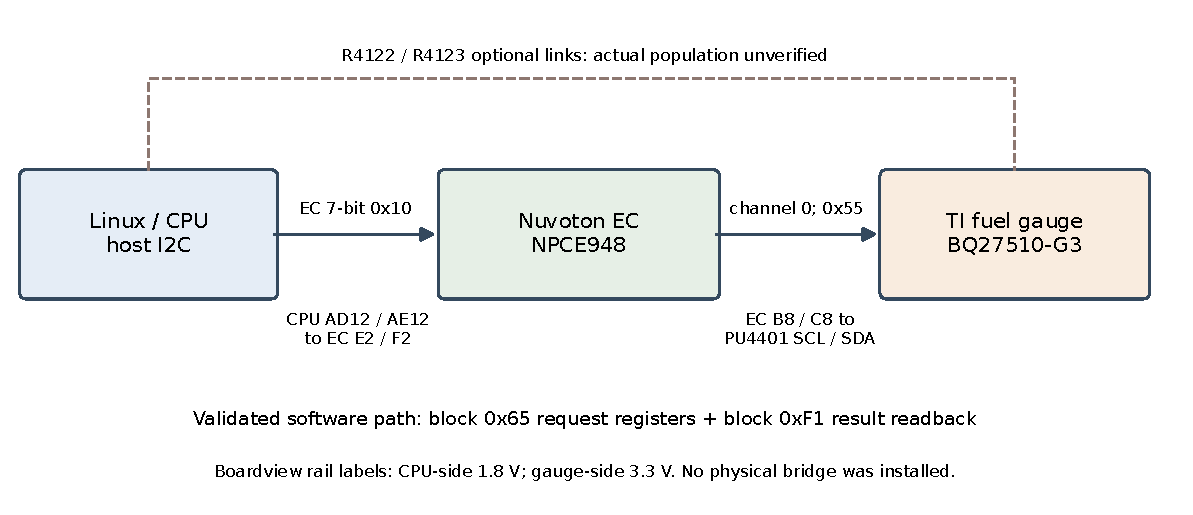
\includegraphics[width=\linewidth]{figures/topology.pdf}
\caption{Access-path reconstruction. Boardview-derived connections suggest separate host-facing and gauge-facing EC segments. The EC address and downstream access were validated in software; physical link population and live rail voltages were not measured. Dashed optional links were not modified.}
\label{fig:topology}
\end{figure}

\section{Stage III: locating executable EC firmware}
\subsection{Approaches that did not establish downstream access}
The DSDT's WMI methods provided an initial service map. Two GUIDs reached \code{WH15}:
\begin{itemize}
\item \code{67C3371D-95A3-4C37-BB61-DD47B491DAAB};
\item \code{431F16ED-0C2B-444C-B267-27DEB140CF9C}.
\end{itemize}
Several subfunctions sent fixed OEM payloads to EC block \hex{61}. However, the AML \code{WRBL} implementation selected only blocks \hex{60}/\hex{61}, and \code{RDBL} also used a bounded switch. This did not establish an arbitrary downstream-address tunnel. No unknown WMI service frame was sent as a trial.

An early, third-party reference SPI image exposed UEFI modules named \code{FotaECUpdate}, \code{I2cKbcDriver}, \code{OememSmiBin}, and \code{OememDxeBin}. The updater contained \code{ECUPDATE.bin} and erase/programming strings, but was host-side update code, not a confirmed executable EC image. Its version and equivalence to the local system were not established. It helped identify the type of missing artifact; none of the final access claims depends on treating that reference dump as authoritative.

SmartBatteryHack~\cite{smartbatteryhack} and DJI firmware tools~\cite{dji} supplied useful examples of battery tooling, but not this EC bridge. A BQ8050-oriented ROM-address sequence using \hex{40} could not safely be transferred to a BQ27510, whose \hex{40}--\hex{5F} range is a DataFlash window. The battery-reset document bundled with the inspected SmartBatteryHack revision describes a BQ2084 procedure, not evidence that a BQ8050 cycle-count change alone restores capacity. These references were inspected statically and were not executed against the target.

\subsection{Official package extraction and identity}
Official A07 and A04 packages were obtained from Dell~\cite{dell-a07,dell-a04,dell-index}. The A04 page was initially inaccessible with HTTP 403; the public driver index supplied its direct download path. Table~\ref{tab:artifacts} records package identity. Neither executable was launched.

\begin{table}[htbp]\centering\small
\begin{tabular}{lll}\toprule
Artifact & Size (bytes) & Role\\\midrule
\code{5055A04.EXE} & 3,615,416 & Official A04 update package\\
\code{5055A07.EXE} & 3,626,376 & Official A07 update package\\
\code{@EC0} decoded component & 131,072 & EC firmware in both packages\\
\code{@R00} decoded component & 6,886,400 & BIOS update component\\\bottomrule
\end{tabular}
\caption{Artifact sizes. Full SHA-256 digests and Dell download URLs are included in Appendix~\ref{app:hashes} and the evidence manifest.}\label{tab:artifacts}
\end{table}

The PE overlay contained an AMI UAF container, identified by \code{@UAF}, followed by tagged modules \code{@UII}, \code{@W32}, \code{@W64}, \code{@R00}, and \code{@EC0}. Module headers supplied sizes and checksum-16 values; compressed modules additionally supplied compressed and original lengths. Bounds, checksums, and decompressed lengths were checked before use. The independently extracted A04 and A07 \code{@EC0} components were byte-identical, with SHA-256 beginning \code{21e4efa3}. This establishes equivalence of those two distributed components, not a complete live-EC readback.

\subsection{Embedded scripts as analysis anchors}
The EC image contained a descriptive string \code{0W.SILV.0X.19} and two continuous FlashStream-like text scripts at file offsets \hex{0F6A6} and \hex{1110A}. Each script was 6755 bytes and 247 lines, containing 162 write operations, 41 comparisons, and 44 delays. Both included hexadecimal data decoding to \code{bq27510-G3}; nearby messages referred to SDI, SIMPLO, update readiness, and flash completion/errors. The scripts included normal-address byte \hex{AA} and address byte \hex{16}, consistent with a normal/programming-address distinction. No script was replayed.

The presence of scripts was initially only a static observation. Direct byte searches for their file offsets failed to find pointer literals. CR16C decoding instead found pointers \hex{2F6A6} and \hex{3110A}: an offset of \hex{20000} from the file positions. This distinction prevented confusing a data pointer with a file offset or a bus address.

\subsection{Reconstructed calling chain}
The subsequent trace established the following path, using file offsets throughout:
\begin{enumerate}
\item A periodic task call at \hex{3E80} reaches \hex{71BC}; for a counter remainder of 199 modulo 500, it calls \hex{7E6A}. The tick duration was not established.
\item The battery-state machine at \hex{7E6A} checks flags at RAM \hex{10468}, queue state, and configuration identifiers. A readiness path calls \hex{83B6}.
\item The executor at \hex{83B6} checks counters and flags. A hardware bit at \hex{FFF251}, bit 5, selects an SDI or SIMPLO script pointer and the common length \hex{1A63}.
\item The call at \hex{8434} reaches parser \hex{81D4}. The parser distinguishes \code{W}, \code{C}, \code{X}, and semicolon-prefixed comments.
\item The write path at \hex{827A} reaches transaction builder \hex{C058}; a descriptor based at \hex{104FC} is passed to engine \hex{A5DE}.
\end{enumerate}

The configuration branch compared observed identifier pairs corresponding to \hex{3352}/\hex{1102} and \hex{3353}/\hex{2202}, in conjunction with the hardware selector. A match sets completion-related bits; a mismatch can lead toward the script executor. Retry and error branches constrain this behavior. We did not induce a mismatch or verify that every statically inferred path executes on this unit.

CR16C instruction semantics required particular care. For example, the inspected SLEIGH definition displays \code{LSHW $0xC} for a shift whose effective count is $12-16=-4$, so the relevant sequence tests flag bit 4, not a twelve-bit left shift. Analysis scripts asserted several call and pointer landmarks and decoded selected regions linearly from function boundaries. A separate every-halfword index was used only for searching; it was not treated as a valid disassembly of all code and embedded data.

\section{Stage IV: identifying the host-facing bridge}
\subsection{From logical registers to the internal engine}
The decisive host path was distinct from directly triggering the embedded programming scripts. In the decoded dispatcher, block \hex{65} accepted a logical-register number and a value, and reached the EC register-write dispatcher at \hex{48FA}. Block reads in the \hex{F0}--\hex{FF} range selected groups of sixteen logical registers through \hex{43DE}. Thus block \hex{F1} exposed logical registers \hex{10}--\hex{1F}.

Logical register \hex{18} triggered a request. Its write path at \hex{4A04} queued a descriptor through \hex{3412}, eventually reaching the same \hex{C058} engine identified from the programming-script path. Completion callback \hex{0F} reached \hex{73C8} and \hex{4D42}, exposing status and clearing the request register. This was a static connectivity hypothesis until exercised on the live target.

\begin{table}[htbp]\centering\small
\begin{tabular}{p{18mm}p{110mm}}\toprule
EC register & Observed role\\\midrule
\hex{17} & Low two bits select the downstream channel; reads also expose live bus-state bits. Channel 0 reached the gauge.\\
\hex{18} & Request protocol and trigger: 6 write byte, 7 read byte, 8 write word, 9 read word, for the paths exercised here.\\
\hex{19} & Completion status; \hex{80} accompanied successful validated operations.\\
\hex{1A} & Target address in eight-bit format; \hex{AA} selected the gauge.\\
\hex{1B} & Downstream register or command.\\
\hex{1C}, \hex{1D} & First two bytes of the request/result data window.\\\bottomrule
\end{tabular}
\caption{Dynamically exercised subset of the logical EC request interface. This is not a specification of every protocol or address supported by the firmware.}\label{tab:registers}
\end{table}

\subsection{Framing and checksums}
A sixteen-byte block read sends a one-byte block selector followed by an eighteen-byte read. Let $b$ be the block command and $P$ the sixteen-byte payload. The response is
\begin{equation}
 [\hex{10},P,c],\quad
 c=\mathrm{CRC8}_{07}([\hex{20},b,\hex{21},\hex{10},P]),
\end{equation}
where CRC-8 uses polynomial \hex{07}, initial value zero, non-reflected processing, and no final XOR.

The logical-register write used in this study sends
\begin{equation}
 [\hex{65},\hex{10},r,v,\underbrace{0,\ldots,0}_{14},c],
\end{equation}
with CRC computed over the EC write-address byte followed by all preceding packet bytes. The payload remains sixteen bytes; $r$ and $v$ occupy its first two positions. This framing was independently consistent with the DSDT's CRC construction and live readback. It must not be confused with a direct gauge write.

For example, the fixed logical-register write selecting gauge address \hex{AA} is:
\begin{lstlisting}
65 10 1a aa 00 00 00 00 00 00 00 00 00 00 00 00 00 00 20
\end{lstlisting}
The first and last bytes here belong to EC command framing and its CRC. They are not the gauge's DataFlash checksum.

\subsection{Dynamic validation and two corrected mistakes}
Initial read-only probes of EC blocks \hex{F1}, \hex{F2}, and \hex{F3} returned valid CRCs. A gauge voltage request then completed with status \hex{80}. The first decoder incorrectly read the result from block \hex{F2} and reported zero voltage. The preserved \hex{F1} reply actually contained bytes \code{94 10} at logical registers \hex{1C}/\hex{1D}, corresponding to 4244 mV. The original failed interpretation and its correction are both retained. Later diagnostic reads independently returned plausible voltage and other gauge values using the correct result location.

A second mistake arose during extended acquisition: a guard treated the entire read value of logical register \hex{17} as a channel number. An otherwise valid reply transiently contained \hex{10}, a live bus-state bit. The tool stopped before triggering the next gauge operation and restored selectors. The corrected version checked the low channel bits separately and waited for the observed bus-state indication to clear. The retained failure is evidence of the guard behavior, not proof that the host can exclude all other bus masters.

The host interface was validated for a fixed set of byte/word operations at one target address. Neither all possible protocol values nor all downstream peripherals were tested. ``Bridge'' in this paper therefore denotes this validated subset, not an experimentally established unrestricted bus proxy.

\section{Stage V: identifying and acquiring the gauge model}
\subsection{Identity and access state}
Live \code{Control()} queries returned DeviceType \hex{0510}, firmware \hex{0400}, ChemID \hex{3353}, and DataFlash version \hex{2202}. Control status \hex{028B} had SS/FAS bits clear under the documented layout. No key submission or security-state transition was required. These observations do not establish the production default state of other units.

There is a documentation discrepancy worth retaining: the downloaded TRM's identity examples name \hex{0520} and \hex{0329}, whereas this device returns \hex{0510}/\hex{0400}. Attribution to the BQ27510-G3 is supported jointly by boardview component naming, the firmware/configuration strings, the acquired field layout, and the runtime identity; it is not based on forcing returned values to match examples.

\subsection{DataFlash acquisition}
The interface acquired class/block data through the gauge's selection registers and read its thirty-two-byte window. Each accepted block satisfied
\begin{equation}
 c_{\mathrm{DF}}=(255-\sum_{i=0}^{31}d_i)\bmod256.
\end{equation}
This byte-complement checksum is distinct from transport CRC-8. During acquisition, the tool wrote class/block and access-mode selectors but never the payload window or checksum-commit register.

The consolidated acquisition contains 25 blocks (800 bytes): classes 2, 32, 34, 36, 48, 49, 64, 68, 81, 82, 83, 84, 87, 88, 91--94, 104, and 107 at block 0; class 80 at blocks 0--2; and class 106 at blocks 0--1. Three valid blocks came from the first, interrupted session and twenty-two from the completed session. Both sessions verified restoration of gauge selectors and EC request fields. This is a selected, documented-configuration backup, not a complete instruction-memory or reserved-DataFlash dump. The complete blocks later considered for modification were included.

\subsection{Configuration and learned state}
Table~\ref{tab:model} summarizes fields derived from checksum-verified blocks. The stored default profiles both contained Qmax 8794 mAh and the same ChemID as the active model. We call these \emph{device-resident reference profiles}: they are not a freshly measured reference cell or a recovered manufacturing-time record.

\begin{table}[htbp]\centering\small
\begin{tabular}{lll}\toprule
Quantity & Observed value & Location\\\midrule
Design capacity & 8680 mAh & Class 48, offset 10\\
SOH reference load & $-400$ mA & Class 48, offset 13\\
Qmax0 / Qmax1 & 7720 / 7869 mAh & Class 82, offsets 2 / 7\\
Cycle count0 / count1 & 49 / 17 & Class 82, offsets 4 / 9\\
UpdateStatus0 / status1 & 2 / 2 & Class 82, offsets 6 / 11\\
Default Qmax0 / Qmax1 & 8794 / 8794 mAh & Classes 83 / 84, offset 2\\
Load mode / select & 1 / 1 & Class 80, offsets 0--1\\
Terminate voltage & 3420 mV & Class 80, offset 46\\
Reserve charge / energy & 0 / 0 & Class 80, offsets 59 / 61\\
Charging voltage & 4350 mV & Class 34, offset 2\\
Taper current & 421 mA & Class 36, offset 2\\
Quit current & 40 mA & Class 81, offset 4\\
SystemDown threshold & 3517 mV & Class 49, offset 5\\\bottomrule
\end{tabular}
\caption{Selected measured model fields. ``Location'' gives decimal class numbers and byte offsets, not I$^2$C addresses. Load mode is offset 1 and load select offset 0.}\label{tab:model}
\end{table}

The active profile indicator was zero. Its resistance columns were classes 91 and 93; the latter carried flag \hex{55}. Both columns were backed up because the firmware can alternate storage columns. Default resistance profiles were classes 87/88. We decompressed the acquired tables using the documented cumulative BaseR-plus-delta representation~\cite{ti-theory}. Figure~\ref{fig:resistance} presents native table units, avoiding an unverified conversion to room-temperature milliohms. Learned profile-0 values were above the resident reference values at the displayed points. Such differences can be consistent with aging or model history; they do not prove corruption.

\begin{figure}[htbp]\centering
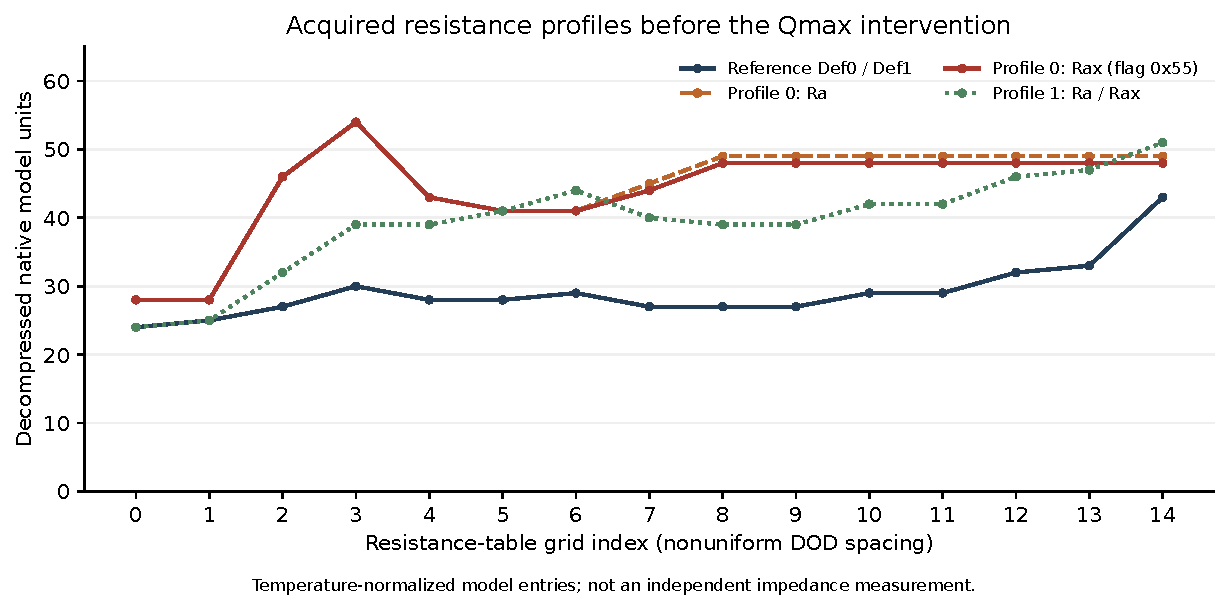
\includegraphics[width=0.91\linewidth]{figures/resistance.pdf}
\caption{Measured resistance-table comparison after decompression. Grid index is not linearly spaced state of charge; values are shown in native encoded-model units with temperature normalization, not as independently measured resistance.}\label{fig:resistance}
\end{figure}

\section{Stage VI: a bounded Qmax intervention}
\subsection{Hypothesis and authorized scope}
The intervention asked whether changing one stored model input, followed by gauge reinitialization, would change reported capacity without changing the cycle count or learned resistance blocks. It did not test electrochemical rejuvenation. The owner explicitly authorized replacing active-profile Qmax 7720 mAh with 8794 mAh from the unit's own reference profile, one gauge reset, and post-operation verification.

The cycle-count-only hypothesis discussed earlier was not tested. The intervention did not set either cycle counter to zero or one. Nor was the proposed broader relearning/reference-resistance reset executed. Those prospective variants must not be conflated with the completed experiment. Manufacturer learning-cycle guidance~\cite{ti-learning} informed the prospective plan but no qualifying learning cycle was performed.

\subsection{Fresh acquisition and transaction sequence}
The experiment beginning at 20:36:05 UTC first checked the product/board/BIOS identity, accessible EC interface, gauge identity tuple, profile indicator, access state, voltage, and temperature. It acquired fresh complete class-82, class-83, class-91, and class-93 blocks. The original block files were saved in the diagnostics tree and a second filesystem directory under \code{/var/backups}; correspondence between copies was later verified. These are two locations on the same device, not an off-device disaster-recovery copy.

The candidate class-82 block differed from the fresh original only at offsets 2 and 3. In big-endian representation:
\begin{lstlisting}
Before State block:
01 00 1e 28 00 31 02 1e bd 00 11 02 fa 88 ec 4d
00 35 02 bc 00 14 03 e8 10 f1 10 f7 00 00 00 00
After State block:
01 00 22 5a 00 31 02 1e bd 00 11 02 fa 88 ec 4d
00 35 02 bc 00 14 03 e8 10 f1 10 f7 00 00 00 00
\end{lstlisting}
The previous and candidate checksums were \hex{E2} and \hex{AC}. The actual persistent-operation sequence consisted of byte writes at gauge registers \hex{42}=\hex{22} and \hex{43}=\hex{5A}, followed by checksum commit \hex{60}=\hex{AC}. The complete staged window was read before commit. After commit, reselecting and reading the entire class-82 block verified persistence. A single \code{Control()} \hex{0041} reset was then issued. No EC/BIOS update command or vendor programming script was executed.

The post-reset checks confirmed Qmax 8794 mAh, initialization completion, Qmax-update enable, continued selection of profile 0, preservation of class-82 bytes outside offsets 2--3, and byte-identical class-91/class-93 resistance blocks. No host write targeted calibration or charging settings. A fresh readback of every other persistent class was not performed, so the claim about untargeted classes is about transaction scope, not an exhaustive post-reset memory attestation.

An error path was prepared to restore the fresh original state if commit verification or the tested postconditions failed. It was not exercised because the checks passed. Its existence is not evidence of tested recovery from interrupted programming, and no power-loss recovery experiment was conducted.

\subsection{Observed reporting changes}
Table~\ref{tab:result} reports the immediate before/after snapshots, also shown in Figure~\ref{fig:results}. The firmware/gauge-reported FCC increased by 854 mAh, or 14.30\% relative to its previous value. SOH rose by 17 percentage points. The two post-intervention health percentages remained different: FCC/design capacity was 78.65\%, whereas the independent SOH register reported 95\%.

\begin{table}[htbp]\centering
\begin{tabular}{lrr}\toprule
Quantity & Before & After reset\\\midrule
Active-profile Qmax (mAh) & 7720 & 8794\\
FCC (mAh) & 5973 & 6827\\
FCC/design capacity (\%) & 68.81 & 78.65\\
SOH (\%) & 78 & 95\\
SOH status byte & 1 & 1\\
Cycle count & 49 & 49\\
SOC (\%) & 97 & 92\\
Voltage (mV) & 4213 & 4213\\
Temperature (\textdegree C) & 27.55 & 26.85\\
Active profile & 0 & 0\\
Control status & \hex{028B} & \hex{028D}\\\bottomrule
\end{tabular}
\caption{The single completed persistent intervention. Temperatures are converted from the recorded tenth-kelvin words using 273.15 K. The post-reset snapshot is not a long-term capacity measurement.}\label{tab:result}
\end{table}

\begin{figure}[htbp]\centering
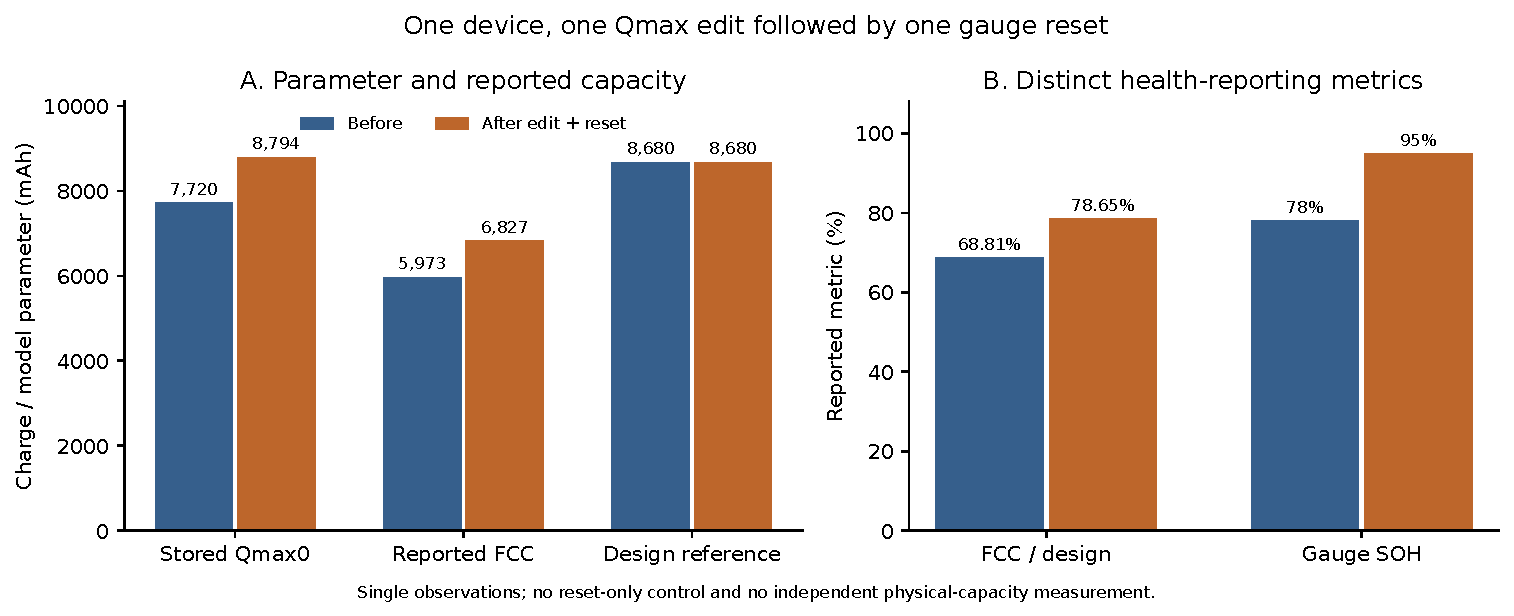
\includegraphics[width=\linewidth]{figures/reporting-change.pdf}
\caption{Reporting before and after the combined Qmax-change/reset intervention. Left: model parameter, reported FCC, and unchanged design reference. Right: two distinct reporting metrics, FCC/design and gauge SOH. These bars are single observations, not sample means or independent measures of physical recovery.}\label{fig:results}
\end{figure}

The SOC change from 97\% to 92\% is a reporting recomputation during reinitialization, not evidence that five percent of the stored charge was consumed during the operation. Control status changed from \hex{028B} to \hex{028D}; QEN remained set and RUP\_DIS became set. We did not wait through a subsequent learning cycle to establish its later trajectory. SOH status remained 1, an instantaneous-result status rather than a newly completed independent aging measurement.

\subsection{What the intervention does and does not establish}
The observations demonstrate that the software path could modify and verify the selected persistent parameter, and that the combined parameter-change/reset procedure was followed by changed gauge outputs while the measured cycle and resistance fields were preserved. The effect of Qmax alone is not isolated: there was no reset-only control, no randomized order, and no return-to-baseline arm. Resetting the gauge can change volatile state and output filtering even when persistent tables remain unchanged. Temperature also differed slightly between snapshots.

Consequently, it would overstate the evidence to report ``a 14.30\% physical capacity recovery,'' or even to assign the entire reporting increase uniquely to the two changed Qmax bytes. The more defensible result is a 14.30\% change in \emph{reported} FCC after a bounded, audited intervention consisting of that edit plus reset. The device was left at Qmax 8794 mAh after the successful test; a subsequent reversion or long-term discharge validation is not part of this record.

\section{Interpretation and implications}
\subsection{Three distinct causes of a misleading health report}
This case exposes three layers that should not be merged into a single wear-level explanation. First, an ACPI method supplied charge as voltage. Second, the operating-system capacity denominator was inconsistent with direct EC information until the reboot, for a refresh reason not isolated here. Third, changing a fuel-gauge model input changed estimates without changing the physical battery.

The initially observed 173\% was therefore not a physically meaningful battery state, and the later 95\% SOH is not a physical restoration certificate. Even after correcting transport and interpretation errors, gauge output remains an estimate contingent on model state. A historical ``wear'' percentage can change because the denominator, model inputs, or measurement conditions changed, not solely because the cells changed.

\subsection{Why a cycle counter is not a capacity proof}
The completed experiment preserved the active counter at 49 while both FCC and SOH changed. It therefore demonstrates that, on this observed path, a capacity-reporting change did not require a cycle-count edit. It does not establish that cycle count has no direct or indirect firmware effects in all circumstances. Nor does it resolve anecdotes from a different BQ8050 firmware family. Algorithm status, cycle count, learned chemical capacity, and resistance profiles are different pieces of state; their register names must not substitute for experimental controls.

\subsection{Repair and driver-development relevance}
The validated interface provides a potential foundation for targeted telemetry tooling or an EC-aware Linux transport layer. An eventual driver would need resource arbitration with platform firmware, robust handling of changing adapter numbering, and a well-defined supported-device match. The userland lock in this study is not sufficient evidence that those kernel-integration questions are solved.

A separate low-risk software repair is the ACPI voltage-source correction. It can be evaluated without changing learned battery parameters. The early-boot override here was scoped to a specific table and boot entry; it did not flash the firmware or establish a generic, permanently supported fix for future kernels and BIOS revisions. Remaining invalid-rate warnings and the earlier full-capacity refresh issue were not fully diagnosed.

\section{Limitations and threats to validity}
\paragraph{Single subject and firmware scope.} One device and one attached battery were studied, with no repeated-unit validation. The same \code{@EC0} bytes in two vendor packages improve confidence in code reuse between those packages but do not prove applicability across every Venue 5055 assembly or firmware version. The live EC's full executable image was not read back.

\paragraph{Physical topology.} Boardview connectivity describes a design. Optional resistor population, live bus voltages, electrical waveforms, and actual component markings were not measured. Negative direct-address probes support, but do not uniquely establish, an isolated physical topology.

\paragraph{Static analysis coverage.} Only relevant slices of proprietary EC code were reconstructed. No whole-program proof, complete interrupt analysis, or formal verification was performed. The inferred automatic programming path was not deliberately triggered, and no security vulnerability or unrestricted downstream-address access is claimed.

\paragraph{Acquisition timing.} The 25-block DataFlash collection spans multiple minutes and two sessions; it is not an atomic memory snapshot. Natural firmware updates could occur between blocks. This is why the persistent experiment reacquired its target and comparison blocks immediately before constructing a candidate.

\paragraph{Measurement versus estimation.} There was no independent coulomb-counter, battery analyzer, controlled run-time test, or energy integration. Resistance values are decoded model entries, not direct impedance spectroscopy. Apparent Qmax retention and FCC/design retention should not be reported as calibrated physical state of health.

\paragraph{Intervention controls.} One Qmax-change/reset sequence was run. A reset-only baseline, sham write, repeat measurements under standardized load, and an A--B--A sequence remain future work. An asserted recovery branch was not exercised. The immediate output could evolve as filtering and learning proceed.

\paragraph{Access and coordination.} The study used an already privileged host and a gauge reporting unsealed access bits. It did not discover unseal keys or demonstrate remote access. Local locking coordinated only the study's processes, while EC firmware and ACPI could continue normal activity. Live status checks reduce some hazards but do not prove absence of multi-master races.

\paragraph{Interpretive corrections.} The first voltage-result offset and a bus-state guard were initially wrong. Both failures and corrections are retained in the evidence. Some contemporaneous notes describe an earlier, incomplete state of the investigation; the claim-to-evidence map and final intervention report supersede those intermediate conclusions.

\section{Reproducibility and artifact availability}
The accompanying source tree includes: a manifest of 63 exported source artifacts; selected raw acquisition reports; 25 measured DataFlash blocks; before/after intervention blocks; tool snapshots; offline checksum/CRC, diff, and transaction-scope verification; and scripts to regenerate tables and figures. The offline verifier validates 2376 recorded EC reply frames and the two-byte state difference without opening a device node. A valid checksum is a consistency check, not cryptographic attestation of the acquisition process.

Vendor packages must be obtained from their listed Dell URLs and verified against the recorded SHA-256 digests before offline extraction. The package contains neither redistributable copies of those executables nor their full decoded images or a vendor boardview. A minimal extraction tool and input fingerprints let a reader reproduce the relevant analysis locally. The actual device boardview remains owner-supplied; absent lawful access to that source, its full netlist cannot be independently regenerated from the release alone.

Hardware-facing source snapshots are included as experimental artifacts, with their original platform guards and fixed targets, not as a generic battery-repair product. Building the paper, validating evidence, and regenerating figures never invoke them. Hardware reproduction entails additional device-specific and electrical considerations and must be distinguished from offline reproducibility.

The manuscript and data are licensed CC BY 4.0; original project code is MIT-licensed. Third-party sources, firmware, trademarks, and underlying board designs retain their respective rights. The companion repository is \url{https://github.com/kjakobczyk/venue5055-battery-research}. No DOI or arXiv identifier has yet been assigned.

\section{Conclusion}
A layered investigation recovered meaningful battery telemetry despite an ACPI defect and a gauge that did not answer the tested direct host transactions. Official update packages, CR16C analysis, and live protocol checks exposed an EC-mediated access path suitable for the specific diagnostic operations demonstrated. A separately authorized edit of two persistent Qmax bytes, followed by gauge reset, changed reported FCC and SOH while preserving cycle count and measured resistance blocks. The work shows why reliable transport, model interpretation, and physical-capacity validation are separate tasks. It establishes a reproducible access and reporting case study, not a method for physically rejuvenating cells.

\section*{Acknowledgments and use of AI assistance}
The investigation and manuscript were prepared with assistance from OpenAI Codex for exploratory analysis, code generation, and drafting. Measurements and verification claims in this draft refer to the preserved tool records, not to independent human replication. Krzysztof Jakóbczyk is the named author; AI systems are not listed as authors. Final release and submission require the author's review of the manuscript, evidence, and cited sources. No unprovided affiliation, ORCID, funding, or institutional approval is asserted.

\appendix
\section{Artifact fingerprints}\label{app:hashes}
\small
\begin{description}
\item[Dell A04 package, SHA-256:]\hfill\break
\code{45cd5b0ca4356a13cb78bc0f0855bc45ac05e56b0d10f70179ba8cb0713caaf6}
\item[Dell A07 package, SHA-256:]\hfill\break
\code{6626d695b48705a43f63d05ba3f577cdfb14ad99e9118a397b0d029a0001cd6d}
\item[Decoded EC component in both packages, SHA-256:]\hfill\break
\code{21e4efa3f1608539e47e5a8e1511c8f9cd0e3ac4703185555c85363135ab3bd8}
\item[Original DSDT, SHA-256:]\hfill\break
\code{ec4d391774c569d9ba0ec415ecd1d13852402e1ae0465a780de4aa2e2c262fbe}
\item[Patched DSDT, SHA-256:]\hfill\break
\code{e92aa9de72f7944e00ba4252899a66dc010280884e95ffb5d6a38f2fea16ea1a}
\item[Owner-supplied GenCAD source, SHA-256:]\hfill\break
\code{bfd0533a997f8d49f2657e6b1f69e917e08b5017c459151306fd4aca2cb66460}
\end{description}
\normalsize
The minimal AML patch changes offsets \hex{9}, \hex{18}, and \hex{11E40}--\hex{11E43}; length remains 76,670 bytes. Fingerprints identify particular study artifacts and are not compatibility tests for a different device by themselves.

\section{Worked read transaction and failure boundaries}
A voltage read uses the following logical sequence: select channel 0 in EC register \hex{17}; set EC register \hex{1A} to \hex{AA}; set \hex{1B} to gauge command \hex{08}; verify the volatile request fields and bus state; trigger protocol 9 through \hex{18}; wait for completion; require status \hex{80}; and decode \hex{1C}/\hex{1D}. Every host block reply is checked for length and CRC before interpretation. A completed request is not inferred solely from a zero-valued result register.

Initial readback with first data bytes \code{94 10} yields
\begin{equation}
 V=\hex{1094}=4244\ \mathrm{mV}.
\end{equation}
An all-zero \hex{F2} block is not evidence of zero battery voltage because \hex{F2} begins at a different logical-register group. The preserved first-test report and correction illustrate why plausible transport completion and a correctly located result must both be checked.

\section{Compact event chronology}
\begin{longtable}{p{21mm}p{117mm}}
\toprule UTC, 2026-10-31 & Recorded event\\\midrule\endhead
15:40 & EC battery replies disagree with sysfs voltage and cached full capacity; sysfs reports 173\%.\\
15:50 & Reboot verification confirms patched DSDT, correct voltage, and refreshed full capacity.\\
16:02 & Five direct gauge-address voltage probes all fail with errno 121.\\
16:23--26 & A07 offline extraction exposes a 128-KiB EC component and embedded scripts. Filesystem times are supporting chronology, not instrument timestamps.\\
16:38 & First bridged voltage response succeeds; initial result-location interpretation is corrected from raw \hex{F1} data.\\
16:39 & Extended gauge diagnostics identify the device and read standard parameters.\\
16:41 & Three initial DataFlash blocks are acquired and checksummed.\\
17:04 & Expanded acquisition stops on an over-strict EC bus-state guard after three valid blocks; selectors restored.\\
17:06 onward & Corrected acquisition obtains twenty-two further blocks and restores selectors. The directory timestamp marks session start, not each block's acquisition instant.\\
20:30 & Fresh diagnostics again report FCC 5973 mAh and 49 cycles.\\
20:36 onward & Fresh backups, two-byte Qmax edit, checksum commit, one gauge reset, and postconditions yield FCC 6827 mAh and SOH 95\%. Individual bus events do not have separate timestamps.\\\bottomrule
\end{longtable}

\bibliographystyle{unsrtnat}
\bibliography{references}
\end{document}
